\documentclass{article}
\usepackage{CJKutf8}
\usepackage{hyperref}
\usepackage{graphicx}
\usepackage{listings}
\usepackage{amsmath}
\begin{document}
\title{Side Channel Analysis for Bluetooth Low Energy}
\author{Dimitri Lanier, \begin{CJK}{UTF8}{gbsn}邱德东, 吴彦廷\end{CJK}}
\date{\today}
\maketitle

\section{Introduction}

In the Internet of Things (IoT) era, Bluetooth Low Energy (BLE/BTLE) has become a prominent wireless communication technology, playing a crucial role. Although BLE's security and privacy have undergone repeated analyses and improvements, the threat posed by side-channel attacks on BLE devices remains insufficiently understood. The BLE key update protocol contains unexplored side-channel vulnerabilities. Specifically, this protocol generates session keys (SKs) using a fixed Long-Term Key (LTK). If the LTK is compromised, it renders all past and future connection encryption ineffective.
In this document we provide a review of the concept BLE and side channel attacks exposing the interplaying vulnerabilities. We also present a low cost side Channel Experiment on Arduino Uno R3 showing the effectiveness of such an attack.
\section{Side-Channel Attacks on Bluetooth Low Energy}
\subsection{ BLE Pairing and Encryption}
Bluetooth Low Energy (BLE) has become a vital wireless communication technology supporting the IoT paradigm. BLE devices are embedded in and widely used in everyday life, such as in personal computers (PCs), smartphones, smart locks, and tablets. BLE is designed to provide low power consumption while maintaining communication range comparable to classic Bluetooth. BLE achieves security through pairing and link-layer encryption.
The pairing process begins when a central device requests to connect to a peripheral device for the first time. According to the latest BLE standards, there are two pairing methods: Legacy Pairing and Secure Connection Pairing. One goal of pairing is to negotiate a Long-Term Key (LTK), used for future link-layer encryption. Legacy Pairing, used in BLE v4.0 and v4.1 devices, employs a unique key exchange protocol defined by the BLE standard. Devices first generate and exchange a Temporary Key (TK) using specific authentication methods. Then, the central and peripheral devices encrypt random numbers (Mrand and Srand) to establish a shared Short-Term Key (STK). This STK is used to encrypt the current connection during pairing, where the LTK and other keys are distributed. Secure Connection Pairing, introduced in BLE v4.2, supports backward compatibility with v4.0 and v4.1 devices. TK and STK are replaced with Elliptic Curve Diffie-Hellman (ECDH) public-key encryption for distributing the LTK. A Diffie-Hellman Key (DHKey), calculated using the P-256 curve, generates the LTK.

After pairing, the central and peripheral devices share an LTK. If bonding is required, the LTK is stored in the devices secure databases and reused in future connections. To ensure confidentiality and integrity, BLE employs AES-CCM (Counter with CBC-MAC) encryption for communication messages. The key for AES-CCM encryption is the Session Key (SK). To further enhance security, BLE introduces a key update protocol to refresh the SK for every new connection. For encryption, the central and peripheral devices exchange two parameters: Initialization Vector (IV) and Session Key Diversifier (SKD). Both parameters consist of two parts: one from the central device and the other from the peripheral, transmitted via the LL\_ENC\_REQ and LL\_ENC\_RSP Protocol Data Units (PDUs), respectively. The central device generates random IVm and SKDm values and sends them to the peripheral via LL\_ENC\_REQ PDU. Similarly, the peripheral generates random IVs and SKDs values and replies via LL\_ENC\_RSP PDU. Once assembled, IV and SKD are used to generate a new SK through encryption with the LTK and AES-128 algorithm. After SK establishment, the central and peripheral devices initialize link-layer encryption via a three-way handshake (LL\_START\_ENC\_REQ and LL\_START\_ENC\_RSP PDUs). Link-layer encryption uses the IV as the initialization vector and the SK as the encryption key. If a new connection is established, the process repeats.
Pairing establishes a shared key, and link-layer encryption provides message confidentiality. However, BLE’s focus on power optimization may have led protocol designers and manufacturers to prioritize simplicity over security. Over the years, BLE's security and privacy have been repeatedly analyzed and patched. Since BLE devices are often deployed in outdoor IoT environments (e.g., smart locks and cameras), attackers can easily approach target devices. Consequently, investigating whether side-channel attacks, such as electromagnetic or power analysis, offer additional advantages is essential. The process of establishing encrypted connections relies on a key update protocol that refreshes the SK for every new connection using the LTK. If this process is compromised, encryption failure can result, leading to severe issues like eavesdropping. A combined electromagnetic side-channel analysis and sniffing attack can recover the full 128-bit LTK of a BLE network, effective against all pairing methods.
\subsection{A Specific Side-Channel Attack on BLE and Its Principles}
The attack allows an adversary to recover the shared LTK between two paired devices (A and B). Once the LTK is acquired, the adversary can compute the SK, decrypting both future and past communications. The attack is effective for both Legacy Pairing and Secure Connection Pairing.
We assume the system consists of two BLE devices, a central device (A) and a peripheral device (B). These devices are paired and share an LTK for link-layer encryption. The attacker aims to decrypt communications between A and B by passively sniffing data packets. The sniffing device must be within BLE's maximum transmission range (approximately 400 meters for BLE v5.0). The attacker may physically approach the devices to collect electromagnetic (EM) leakage signals. In experiments, the EM probe must be positioned extremely close to the target device (within 0.3 cm). To successfully recover the LTK, the attacker must capture related data packets and EM traces from multiple BLE connections.
BLE’s key update protocol generates the SK by encrypting SKD using the LTK. The attacker exploits this vulnerability as follows: The plaintext components of SKD (SKDm and SKDs) are transmitted in plaintext and can be captured via sniffing techniques. Combining the captured SKD values with the EM traces from the encryption process enables the attacker to recover the LTK using vulnerabilities in AES encryption modes (e.g., ECB mode). The attacker must sniff the following packets: unique access address of the current connection, plaintext SKDm value, and plaintext SKDs value. With these packets, the attacker can reconstruct the full SKD for EM analysis. Once sufficient EM traces are collected, the attacker performs Correlation Electromagnetic Analysis (CEMA) to recover the LTK. The attack targets the first-round SubBytes operation of AES encryption, the only nonlinear step in the process. To reduce complexity, the LTK is divided into 16 bytes, recovered one byte at a time. For non-profiling attacks, the Hamming Weight model is used to recover the LTK byte by byte through CEMA. For profiling attacks, efficient methods like template attacks or deep learning-based approaches can be applied.
\section{Countermeasures Against Side-Channel Attacks on Bluetooth Low Energy}
\subsection{Causes of Side-Channel Vulnerabilities}
The BLE key update protocol contains several inherent design flaws that lead to side-channel vulnerabilities:
\begin{itemize}
    \item Sensitivity of the LTK 
        The LTK serves as the core key for BLE encryption and is used to generate all session keys (SKs). If the LTK is recovered, attackers can decrypt all historical and future communication data.
    \item Plaintext Parameters in the Encryption Protocol
        In the key update protocol, the Session Key Diversifier (SKD) and Initialization Vector (IV) are transmitted in plaintext. This makes it easy for attackers to capture these parameters via sniffing and combine them with electromagnetic traces for analysis.
    \item Electromagnetic Leakage in Embedded Devices 
        BLE devices typically operate on low-power embedded hardware that lacks adequate protection against side-channel attacks. Electromagnetic leakage during AES encryption provides attackers with exploitable entry points.
\end{itemize}
Side-channel attacks can recover the LTK regardless of whether Legacy Pairing or Secure Connection Pairing is used. This is because the key update protocol is designed similarly in both modes. The attack applies to BLE devices implemented on general hardware using open-source BLE protocol stacks (e.g., Nimble). Although dedicated AES hardware implementations increase the difficulty of the attack, it remains feasible. Moreover, side-channel attacks employ passive sniffing and electromagnetic analysis, so devices cannot detect the attacker’s presence.
\subsection{Defense Strategies}
To address the above attacks, defense strategies can be implemented through hardware enhancements, protocol improvements, software optimizations, and runtime detection to improve BLE devices' resilience against side-channel attacks.
\begin{itemize}
    \item \textbf{Hardware Enhancements}  
    Introduce electromagnetic shielding in hardware design to reduce signal leakage during device operation. Integrate dynamic power adjustment techniques to mask power variations during encryption operations.

    \item \textbf{Protocol Improvements}  
    Encrypt the transmission of SKD and IV to fundamentally prevent attackers from obtaining these parameters via sniffing. Introduce randomization operations in the protocol to make encryption inputs less predictable, reducing the accuracy of side-channel analysis.

    \item \textbf{Software Optimizations}  
    Utilize more advanced encryption algorithms, such as highly efficient AES hardware acceleration modules, to minimize leakage during encryption operations. Add noise to encryption operations to obscure leakage signals, making it harder for attackers to extract useful information.

    \item \textbf{Runtime Detection}  
    Deploy runtime security monitoring systems to detect abnormal device behavior, such as frequent connection requests or unauthorized sniffing activities.
\end{itemize}

\section{An Experiment Demonstrating Side-Channel Attacks on Arduino Uno R3}
To demonstrate the real threat that is side channel to IoT we wanted to design a pedagogical experiment that easily be reproduced and shown to computer science student and computer security enthusiast. In order to be able to ba as wide spread as possible (and because of our own budget constraint) we decided to create a protocol for doing a really low cost experiment that will only require an arduinno and a Soft Defined Radion based on a RTL820T2 Chip. These compenent are really cheap and we only pay 250 yuan for all experiment. We chosed to RSA as the key exchange mechanism is still widely used in Legacy Bluetooth stacks and it is easier to understand than Elliptic Curve Diffie Hellman for new students.
\subsection{Understanding the Vulnerability}

In our RSA implementation on the Arduino Uno R3, we utilize the fast exponentiation algorithm, commonly known as the square-and-multiply method, to perform modular exponentiation efficiently. This algorithm computes $c = m^d \mod n$ by iterating over each bit of the private exponent \( d \).

The vulnerability arises from the use of an \texttt{if} condition within the exponentiation loop that depends on the value of each bit of the secret key \( d \). Specifically, the algorithm performs an extra multiplication when a bit of \( d \) is 1 and skips it when the bit is 0. This conditional branching causes variations in the device's power consumption and electromagnetic emissions during execution.

An example of the vulnerable code is:
\begin{lstlisting}[language=C]
unsigned long modular_exponentiation(unsigned long base, unsigned long exponent, unsigned long modulus) {
    unsigned long result = 1;
    base = base % modulus;
    while (exponent > 0) {
        if (exponent & 1) {
            result = (result * base) % modulus; // Conditional multiplication
        }
        exponent = exponent >> 1;
        base = (base * base) % modulus;
    }
    return result;
}
\end{lstlisting}

\subsection{Literature Review}
Originally my plan was to follow this paper instruction : \cite{cheapEM} but after some discussion with a friend that is more into the subject I came to realise that the paper was not enough detailed to be able to reproduce the experiment especially on the hardware part of the antenna.
\subsection{Methodology}
If I wanted to have some result I needed something I can fully controll to be able to interprete the EM (Electromagnetic) signal I would see. Therefore I decided to use an R3 Arduino to run the cryptographic algorithm I ordered a cheap SDR (Software Defined Radio) (~90 yuan) to be able to capture the EM signal and I will use a dipole antenna of 12cm to capture the signal.
The first problem that I encountered is that a classic RSA4096 require to much memory for my arduino to be able to run it, so I decided to use RSA512 intead at least it will give me a proof of concept. I used an existing repository as base for my code \cite{github} I modified the code to be able to do private decryption (essentially I added the private key in the code and added a fast expnonentition depending on the bit of the key (originally the code only allow to take 3 as expononent)). Then I flash the code into the card and went through a bit of debugging using the led of arduino untill I had a code that was correct.
\\
After that I had to deal with the radio part , having no experience in SDR I chosed to use GNU radio because it allows me to have simple interface and still provide flexibility with the python blocks. I used a Waterfall sink to identify the leaking frequancies. This was a tedious task as I went into a lot of false leakage through my analysis, firstly I was sending the signal to the arduino through the USB cable and I was capturing the signal with the SDR on the same computer, this was creating a lot of noise in the signal. I was transmiting the signal at baud 9800 and I was able to see the leakage at 29kHz at first I mistook it for the signal I was looking , but the 29MHz didn't make sense since the clock was 16MHz , so i continued investigating, found that my sdr didn't dtect the signal below 20MHz and finally found some interesiting signal at the multiple of 16MHz. 
After examining the Waterfall sink I decided to be really centered on the 4 times the clock frequency with sampling rate of 5kHz. To make this choice I based my self on basic physics our antenna is 12cm and is placed over an conductor plane that make it appear in EM world as if it was 24cm. From this size and the formula $f = \frac{c}{\lambda}$ I found that the maximal gain frequency would be at 1.2GHz but my SDR is only able to mix signal up to 200MHz further from 80MHz the signal is polluted by radio station. Given all these information I decided to look for the highest multiple of the frequency below 80MHz and I found that 4 times the clock frequency was the best candidate. I ran a EM power analysis and after several failed attempts (because my laptop charging was generating noise or I made something move that messed the signal ) I added some averanging to lower the noise and end up with this signal that almost perfectly leaked me the secret key.
\begin{figure}[h]
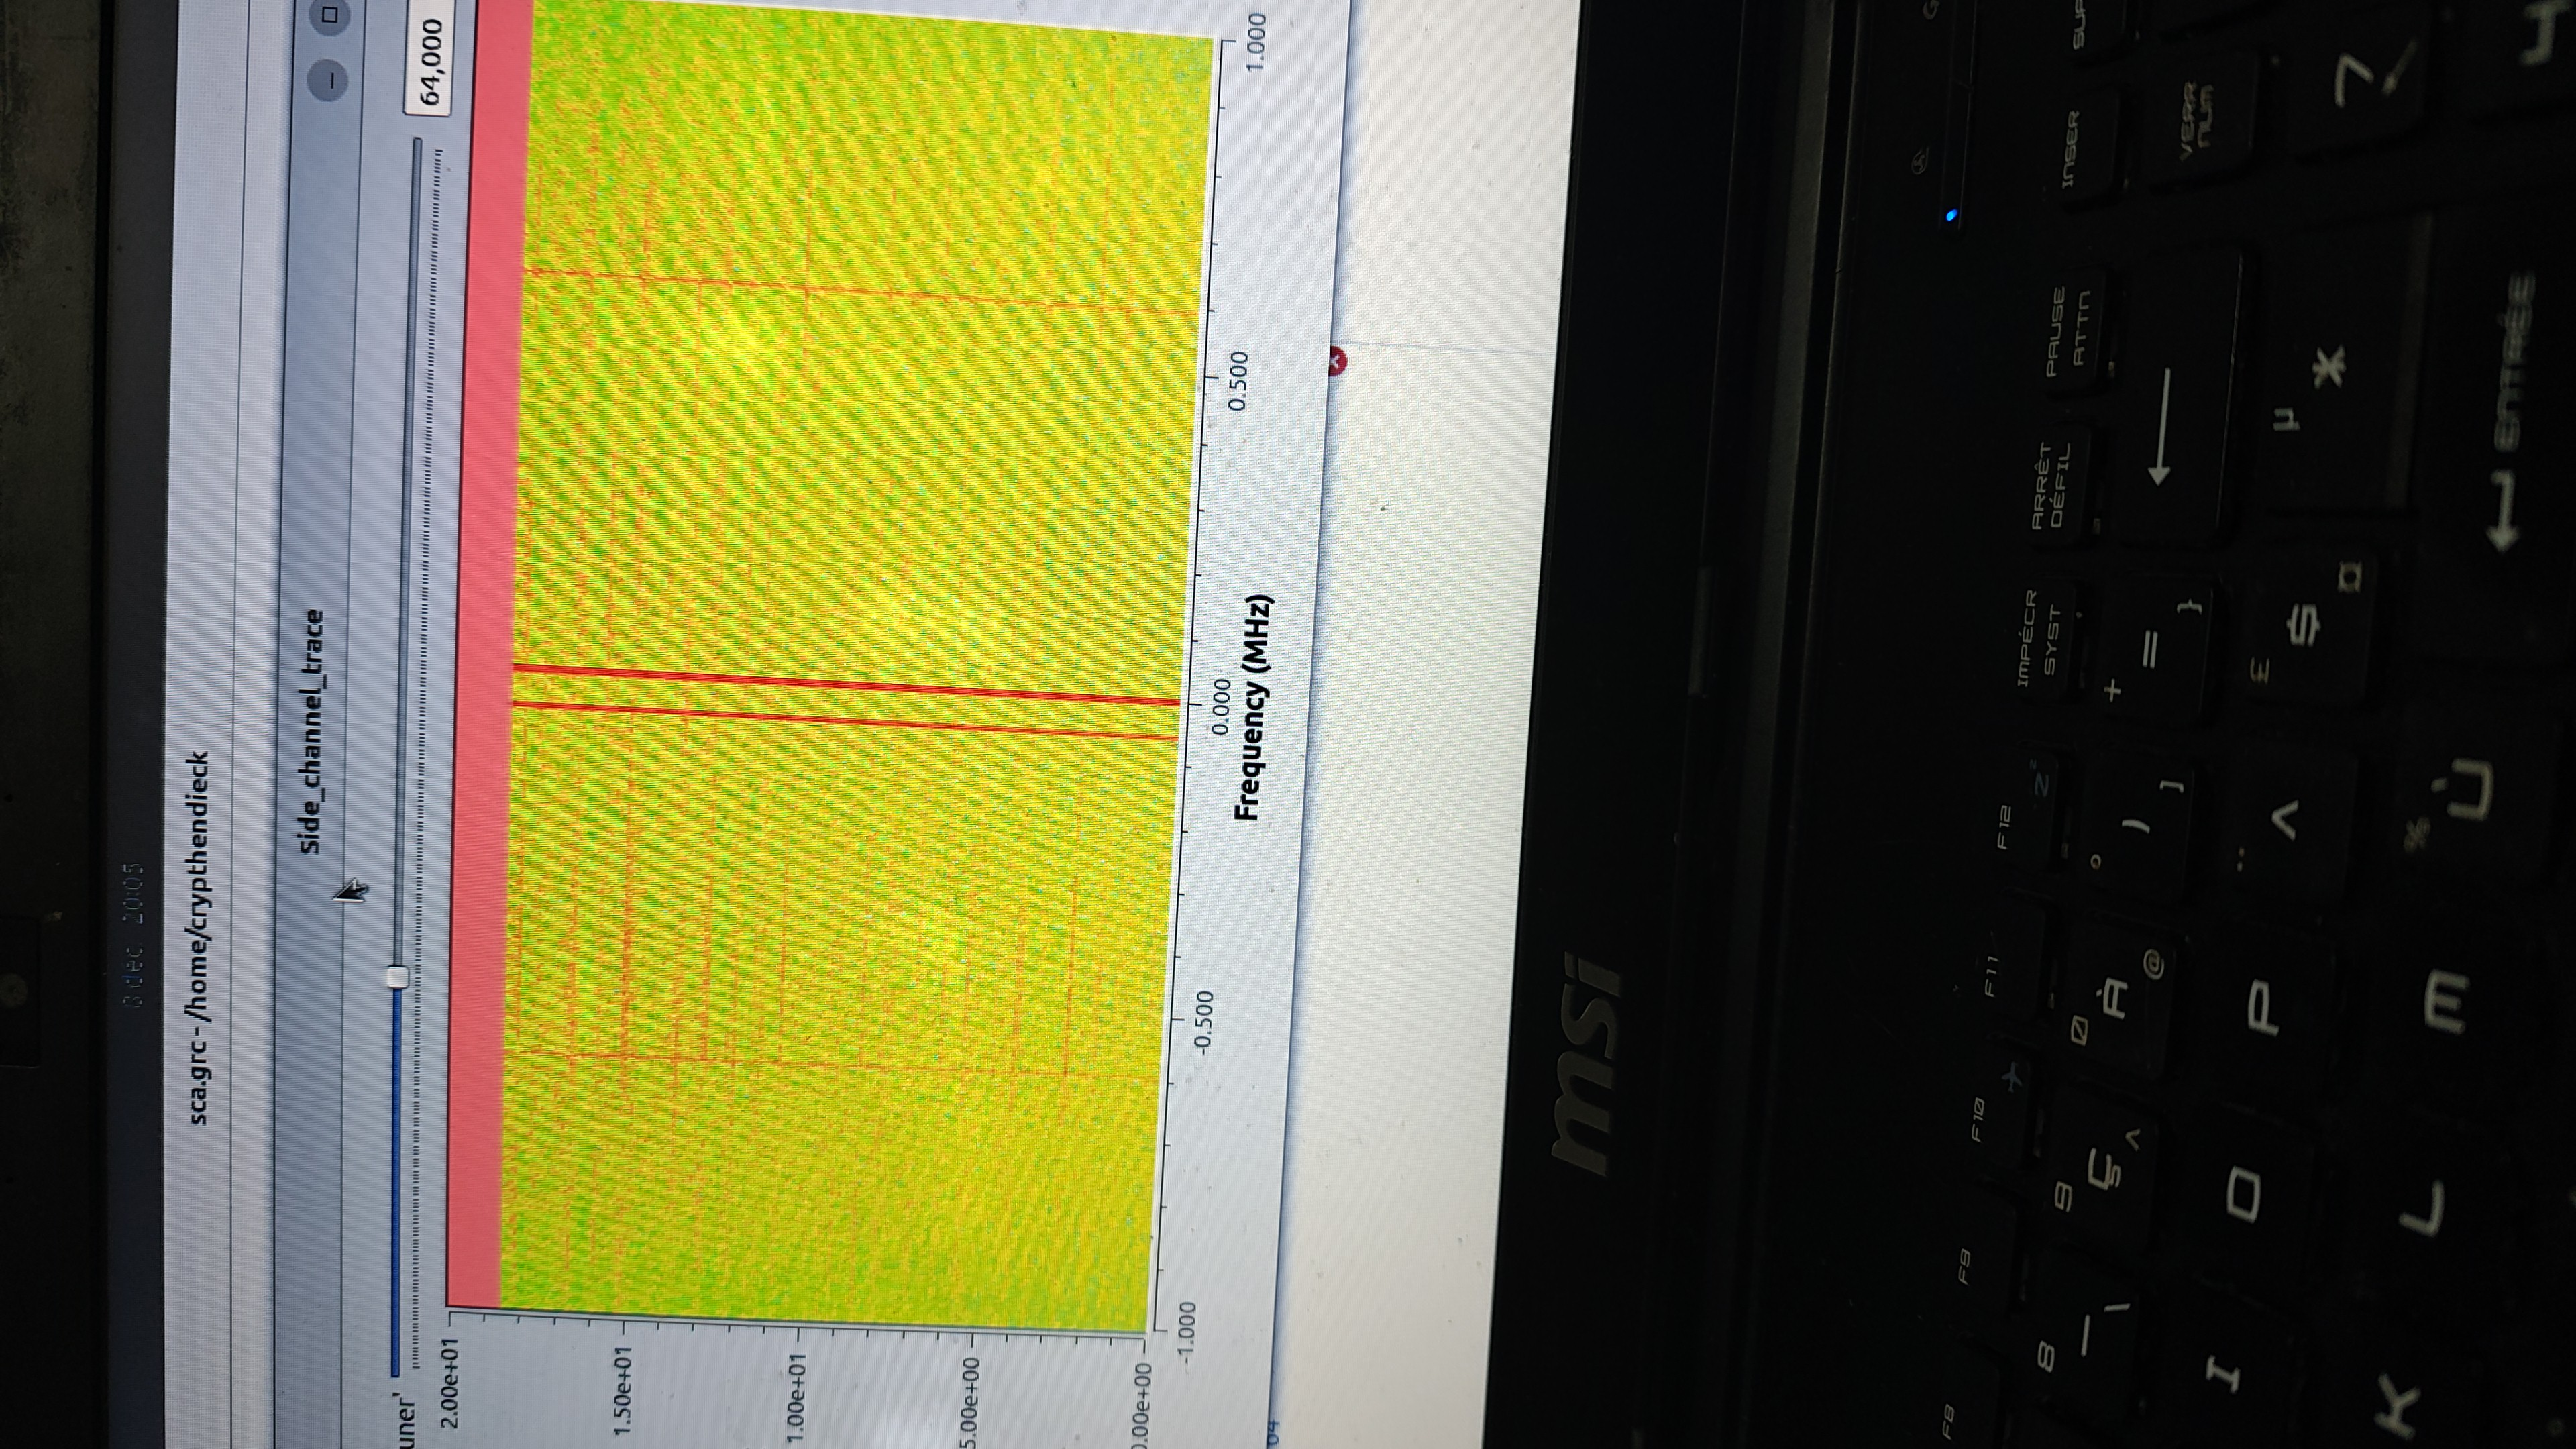
\includegraphics[width=\textwidth]{waterfall.jpeg}
\end{figure}
My final setup looked \begin{lstlisting}[language=C]
    unsigned long modular_exponentiation(unsigned long base, unsigned long exponent, unsigned long modulus) {
        unsigned long result = 1;
        base = base % modulus;
        while (exponent > 0) {
            if (exponent & 1) {
                result = (result * base) % modulus; // Conditional multiplication
            }
            exponent = exponent >> 1;
            base = (base * base) % modulus;
        }
        return result;
    }
    \end{lstlisting}like this , I attached the antenna to the arduino to have better signal and I used a battery to power the arduino to avoid noise from the computer and I stood between my computer and the antenna during the recording to minimize the noise.
\begin{figure}[h]
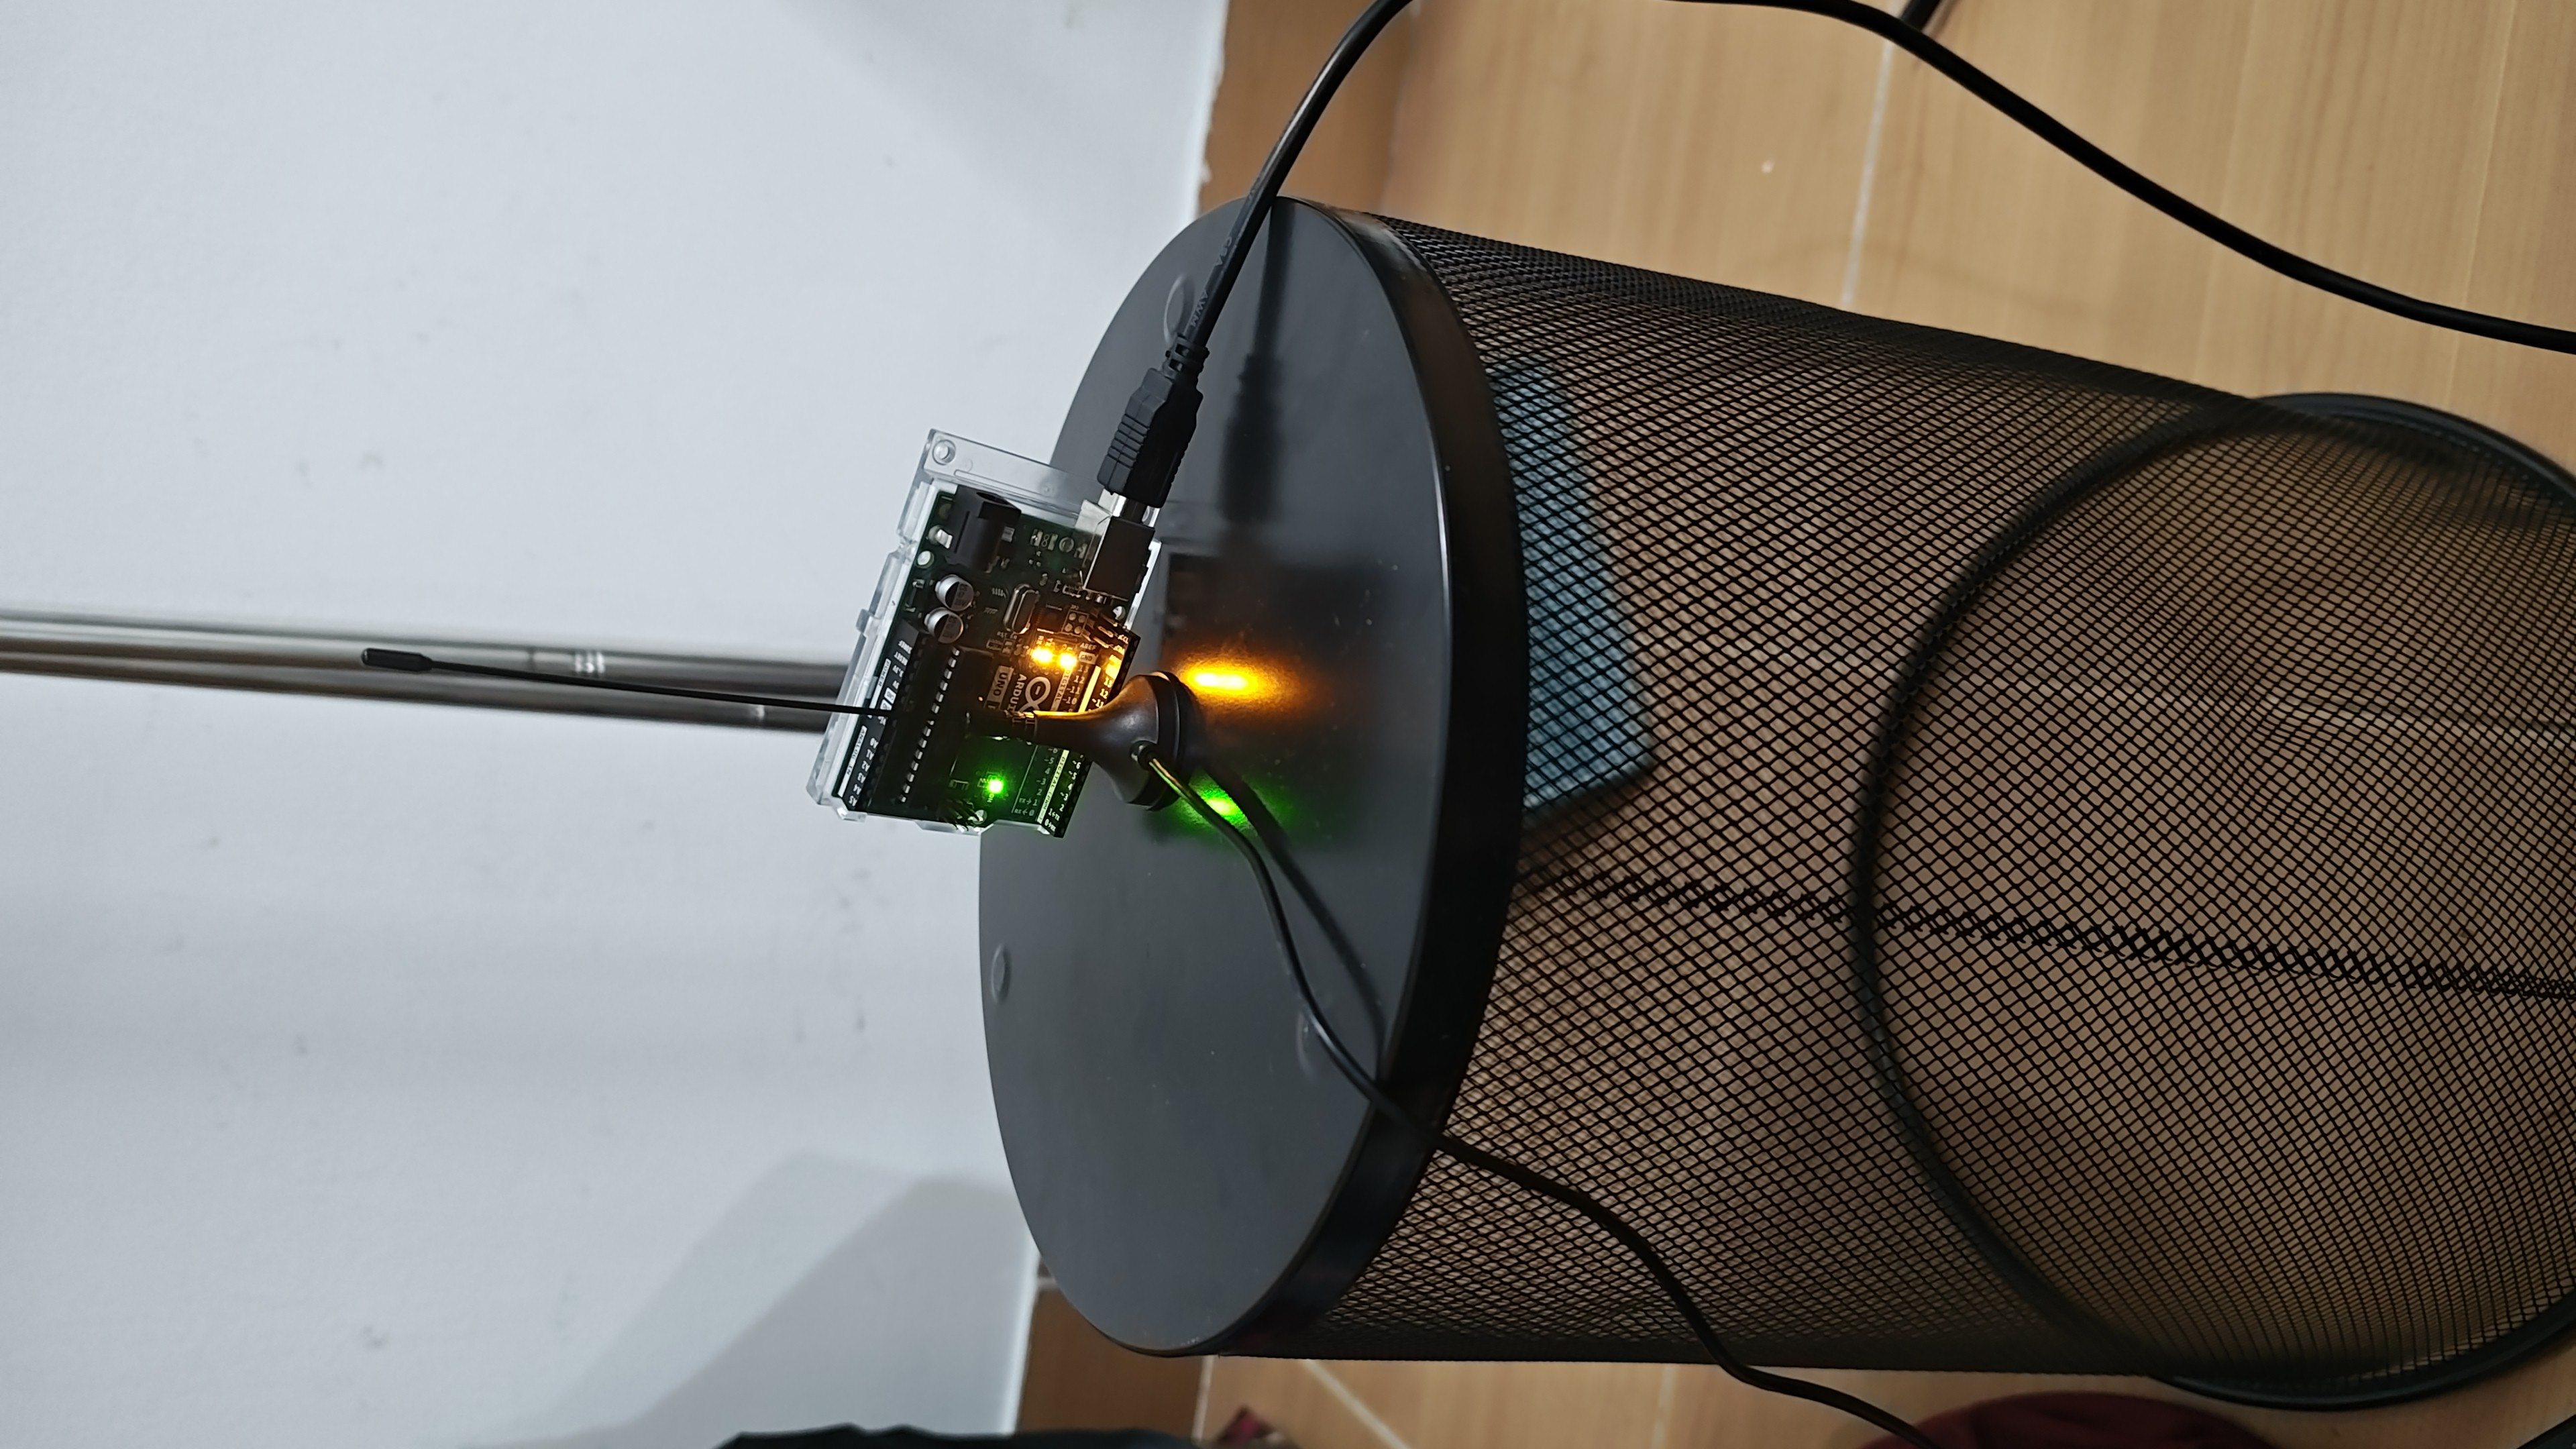
\includegraphics[width=\textwidth]{setup.jpeg}
\end{figure}
\subsection{Results}
To limit the time that took the experiment I choose to take a small secret key, in my experimet my secret key was : $Oxf61d11$ that have $111101100001110100010001$ binary representation.After a power analysis, and moving average to reduce the noise, I was able to recover the secret key with a 91.66\% accuracy. The result of the acquisition is shown in this image.
\begin{figure}[h]
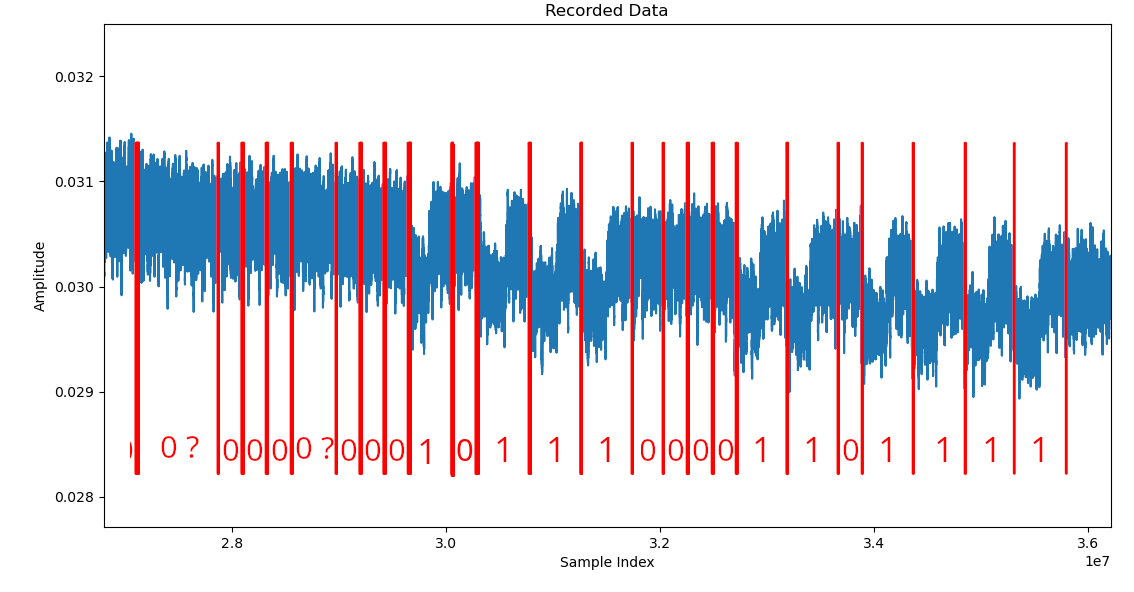
\includegraphics[width=\textwidth]{leaked_secret_key.png}
\end{figure}

\subsection{Discussion}
Discuss the results and their implications here.

\subsection{Conclusion}
Summarize the findings and provide conclusions here.

\begin{thebibliography}{9}

    \bibitem{cheapEM}
    Genkin, Daniel and Pachmanov, Lev and Pipman, Itamar and Tromer, Eran,
    \emph{Stealing Keys from PCs Using a Radio: Cheap Electromagnetic Attacks on Windowed Exponentiation},
    2015, pages 207--228, ISBN 978-3-662-48323-7, DOI \href{https://doi.org/10.1007/978-3-662-48324-4_11}{10.1007/978-3-662-48324-4\_11}.

    \bibitem{github}
    \href{https://github.com/qqqlab/microRSA}{https://github.com/qqqlab/microRSA}

\end{thebibliography}

\end{document}